El siguiente paso consiste en leer los fotones de la luz de centelleo. Para ello, una de las alternativas que contempla nuestro estudio es la utilización de un fotomulitplicador de silicio, que abreviaremos de ahora en adelante  por SiPM. El SiPM es un dispositivo de detección de radiación relativamente nuevo en el mercado, que surge como alternativa al tubo fotomultiplicador. Consiste en una matriz bidimensional formada por multiples pixels independientes y alimentados en paralelo (mismo voltaje operacional para cada uno) a un voltaje tal que les permita funcionar en modo Geiger. Cada uno de los pixels actua como un APD (fotodiodos de avalancha)~\cite{TFMSiPM2}.
Cuando detectan un fotón, estos pixels producen una cascada de pares electrón-hueco, que forman la señal del sistema de detección, la cual estará formada por la suma de las señales de los pixel que han detectado un fotón para cada instante de tiempo. Idealmente, cada pixel únicamente puede detectar un fotón. Si varios fotones caen en el mismo pixel, entonces la señal es más reducida  con respecto de la señal correspondiente a cada fotón en pixeles diferentes.  Esto origina una pérdida de la linealidad de la señal de respuesta con la intensidad de la luz, para intensidades de luz elevadas. Dado que  poseen una alta eficiencia de fotodetección, los SiPM son utilizados como fotosensores, especialmente para señales débiles.
 Los SiPM  poseen una serie de características distintas de los convencionales tubos fotomultiplicadores que los hacen ideales en unas situaciones y no tanto en otras, como por ejemplo su tamaño compacto, inmunidad a campos magnéticos, electrónica sencilla, alta eficiencia de detección de fotones (especialmente adecuado para nuestro experimento), buena linealidad, dependencia con la temperatura significativa, alta ganancia a menor voltaje de alimentación y, por extensión, menor consumo, tiempo de respuesta corto y, por extensión, buena resolución temporal~\cite{AMFNP}.

Hay que tener en cuenta que los SiPM son detectores de estado sólido y, en consecuencia, presentan ruido térmico, ruido que se verá amplificado por el hecho de estar operando en modo Geiger-Muller. Este ruido se denomina corriente oscura (Dark counts) y su forma se ve reflejada en la  figura~\ref{Darkcounts}.

\begin{figure}[hbtp]
\centering
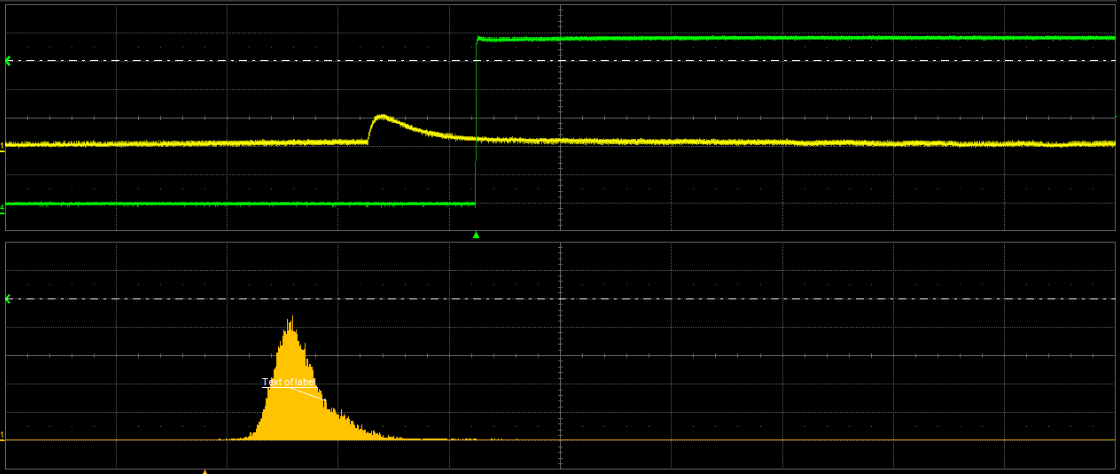
\includegraphics[scale=0.3]{pedestal.png}
\caption{Dark counts\label{Darkcounts}}
\end{figure}

Cuando trabajamos con detectores de estado sólido debemos trabajar en condiciones óptimas de voltaje operacional y temperatura, ya  que las cuentas oscuras dependen de estas magnitudes y pueden llegar a ser tan numerosas que enmascaren por completo la señal que queremos medir. También podemos reducir su importancia sobre la medida con ayuda de triggers, por ejemplo, medir únicamente cuando la señal de entrada del sistema este activa (si se conoce este intervalo de tiempo). En cualquier caso, siempre se deberá realizar una medida del pedestal (señal de respuesta para señal de entrada nula) para tener en cuenta el número y características de los eventos que van a producir una señal sin corresponder a los sucesos que deseamos medir, y utilizar esta información para el posterior análisis. 

En esta sección, desarrollamos un método de compensación para las variaciones de la ganancia de un fotomultiplicador de silicio producidas por variaciones  de la temperatura y del voltaje de alimentación del SiPM (voltaje de polarización inversa), de ahora en adelante llamado voltaje operacional. 

En concreto, utilizaremos el modelo S13360-1375CS de Hamamatsu Photonica. Se ha elegido este modelo debido a que presenta una eficiencia de fotodetección máxima entorno a los $450~\nm$, que corresponde aproximadamente a la longitud de onda del azul, $435~\nm$ y, en concreto, se asemeja bastante con el máximo de la energía reemitida por las fibras centelleadoras BCF-12, $435~\nm$, encargadas de detectar la radiación $\beta$ del agua tritiada en nuestro experimento, como puede apreciarse en la  figura~\ref{Espectros}. De esta forma conseguiremos que la señal sea tan grande como sea posible, algo fundamental ya que, como ya se ha mencionado, una de las principales dificultados del experimento es que estamos intentando medir una señal muy pequeña.

\begin{figure}[htb]
\centering
{
%\subfloat[PDE]
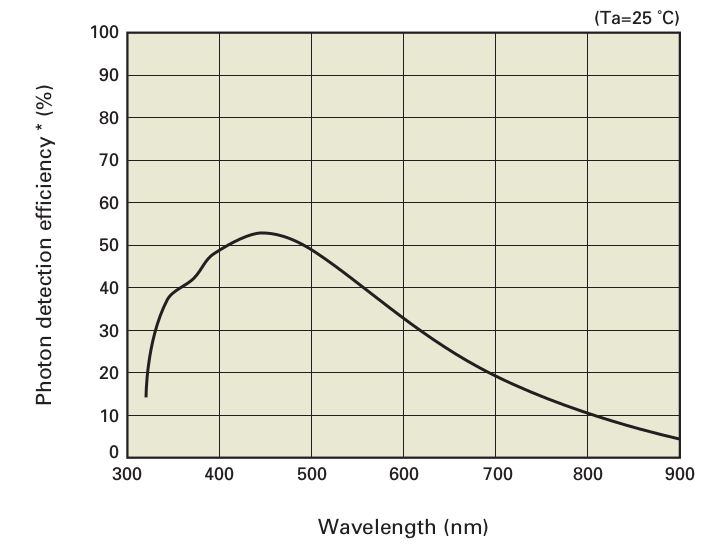
\includegraphics[scale=0.3]{PED.png} 
}
{
%\subfloat[Espectro de emisión]
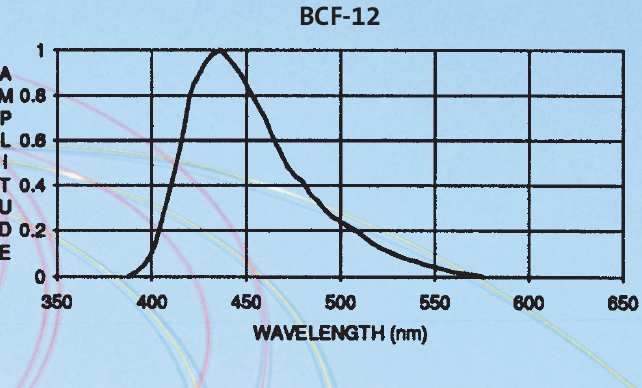
\includegraphics[scale=0.35]{EmisionBCF12.png} 
}
\label{8}
\caption{PDE del SiPM~\cite{datasheet SiPM} y espectro de emisión de las fibras~\cite{datasheet} respectivamente\label{Espectros}}
\end{figure}

La forma de abordar este método de compensación de la ganancia ha sido el siguiente:
\begin{enumerate}
\item {} 
Por un lado se ha realizado una calibración de la ganancia frente a la temperatura, obteniendo su relación de dependencia. Para ello, se ha necesitado la utilización de un sistema de control de temperatura. En concreto se ha utilizado un sistema de la marca DYCOMETAL, (modelo CCM 81), que permite controlar temperatura y humedad relativa con una precisión de $0.1~\celsius$   y  $0.5$\% respectivamente.

\item {} Por otro lado se ha realizado una calibración de la ganancia frente al voltaje operacional, obteniendo su relación de dependencia. Para obtener este voltaje operacional se ha utilizado un electrómetro KEITHLEY, modelo 6517B, el cual presenta una resolución inferior al $\milli\volt$, más que suficiente en nuestro caso ya que se necesitan mayores variaciones para modificar apreciablemente  la ganancia.

\item {} Finalmente, a partir de estas dos dependencias determiandas, se ha obtenido la ecuación de dependencia entre voltaje operacional y temperatura correspondiente a una ganancia constante,  y se ha realizado un test de comprobación de esta relación.
\end{enumerate}

El objetivo final de este estudio será mantener la ganancia del fotomultiplicador de silicio constante ante variaciones involuntarias de la temperatura mediante variaciones controladas del voltaje operacional. Esta es una corrección fundamental para el objetivo final del detector, ya que, de lo contrario, obtendríamos alertas de fugas de tritio cuando estas no han ocurrido, y viceversa,  cuando, en realidad, lo único que ha ocurrido ha sido una modificación de temperatura del detector